\documentclass[a4paper]{article}

\usepackage[english]{babel}
\usepackage[utf8]{inputenc}
\usepackage{amsmath}
\usepackage{graphicx}
\usepackage[colorinlistoftodos]{todonotes}
\usepackage[export]{adjustbox}[2011/08/13]
\usepackage{float}
\usepackage{bm}

\title{Behaviour Dynamics in Social Networks - Assignment 6}

\author{Maria Hotoiu, Federico Tavella}

\date{\today}

\begin{document}
\maketitle

\begin{abstract}
In this assignment the idea is to teach you how to work with social analysis software and data mining with social media data.
\end{abstract}

\section{Part A: Getting data from Social web media}

\subsection{Activity 1}

In the file \emph{home\_timeline.jsonl} there is my personal timeline (i.e. tweets about people that I am following) from Twitter and all the informations related to their profiles. I can retrieve my own tweets looking at the attribute \emph{screen\_name}. The code is parsing my timeline, obtaining informations and meta-data about the tweets contained in it and the related profiles.

Looking at the hashtags I can have an insight to events and locations related to the analyzed profile.

\subsection{Activity 2}

We chose the Twitter profile of Bill Gates because we thought that it could have had a large amount of different hashtags. It is interesting to find about that the  most common hashtags and words are referred to his commitment to defeat diseases such as polio and malaria through the Melinda and Bill Gates Foundation. It would be interesting to see the distribution of these tags over the time.

\begin{figure}[!htpb]
\centering
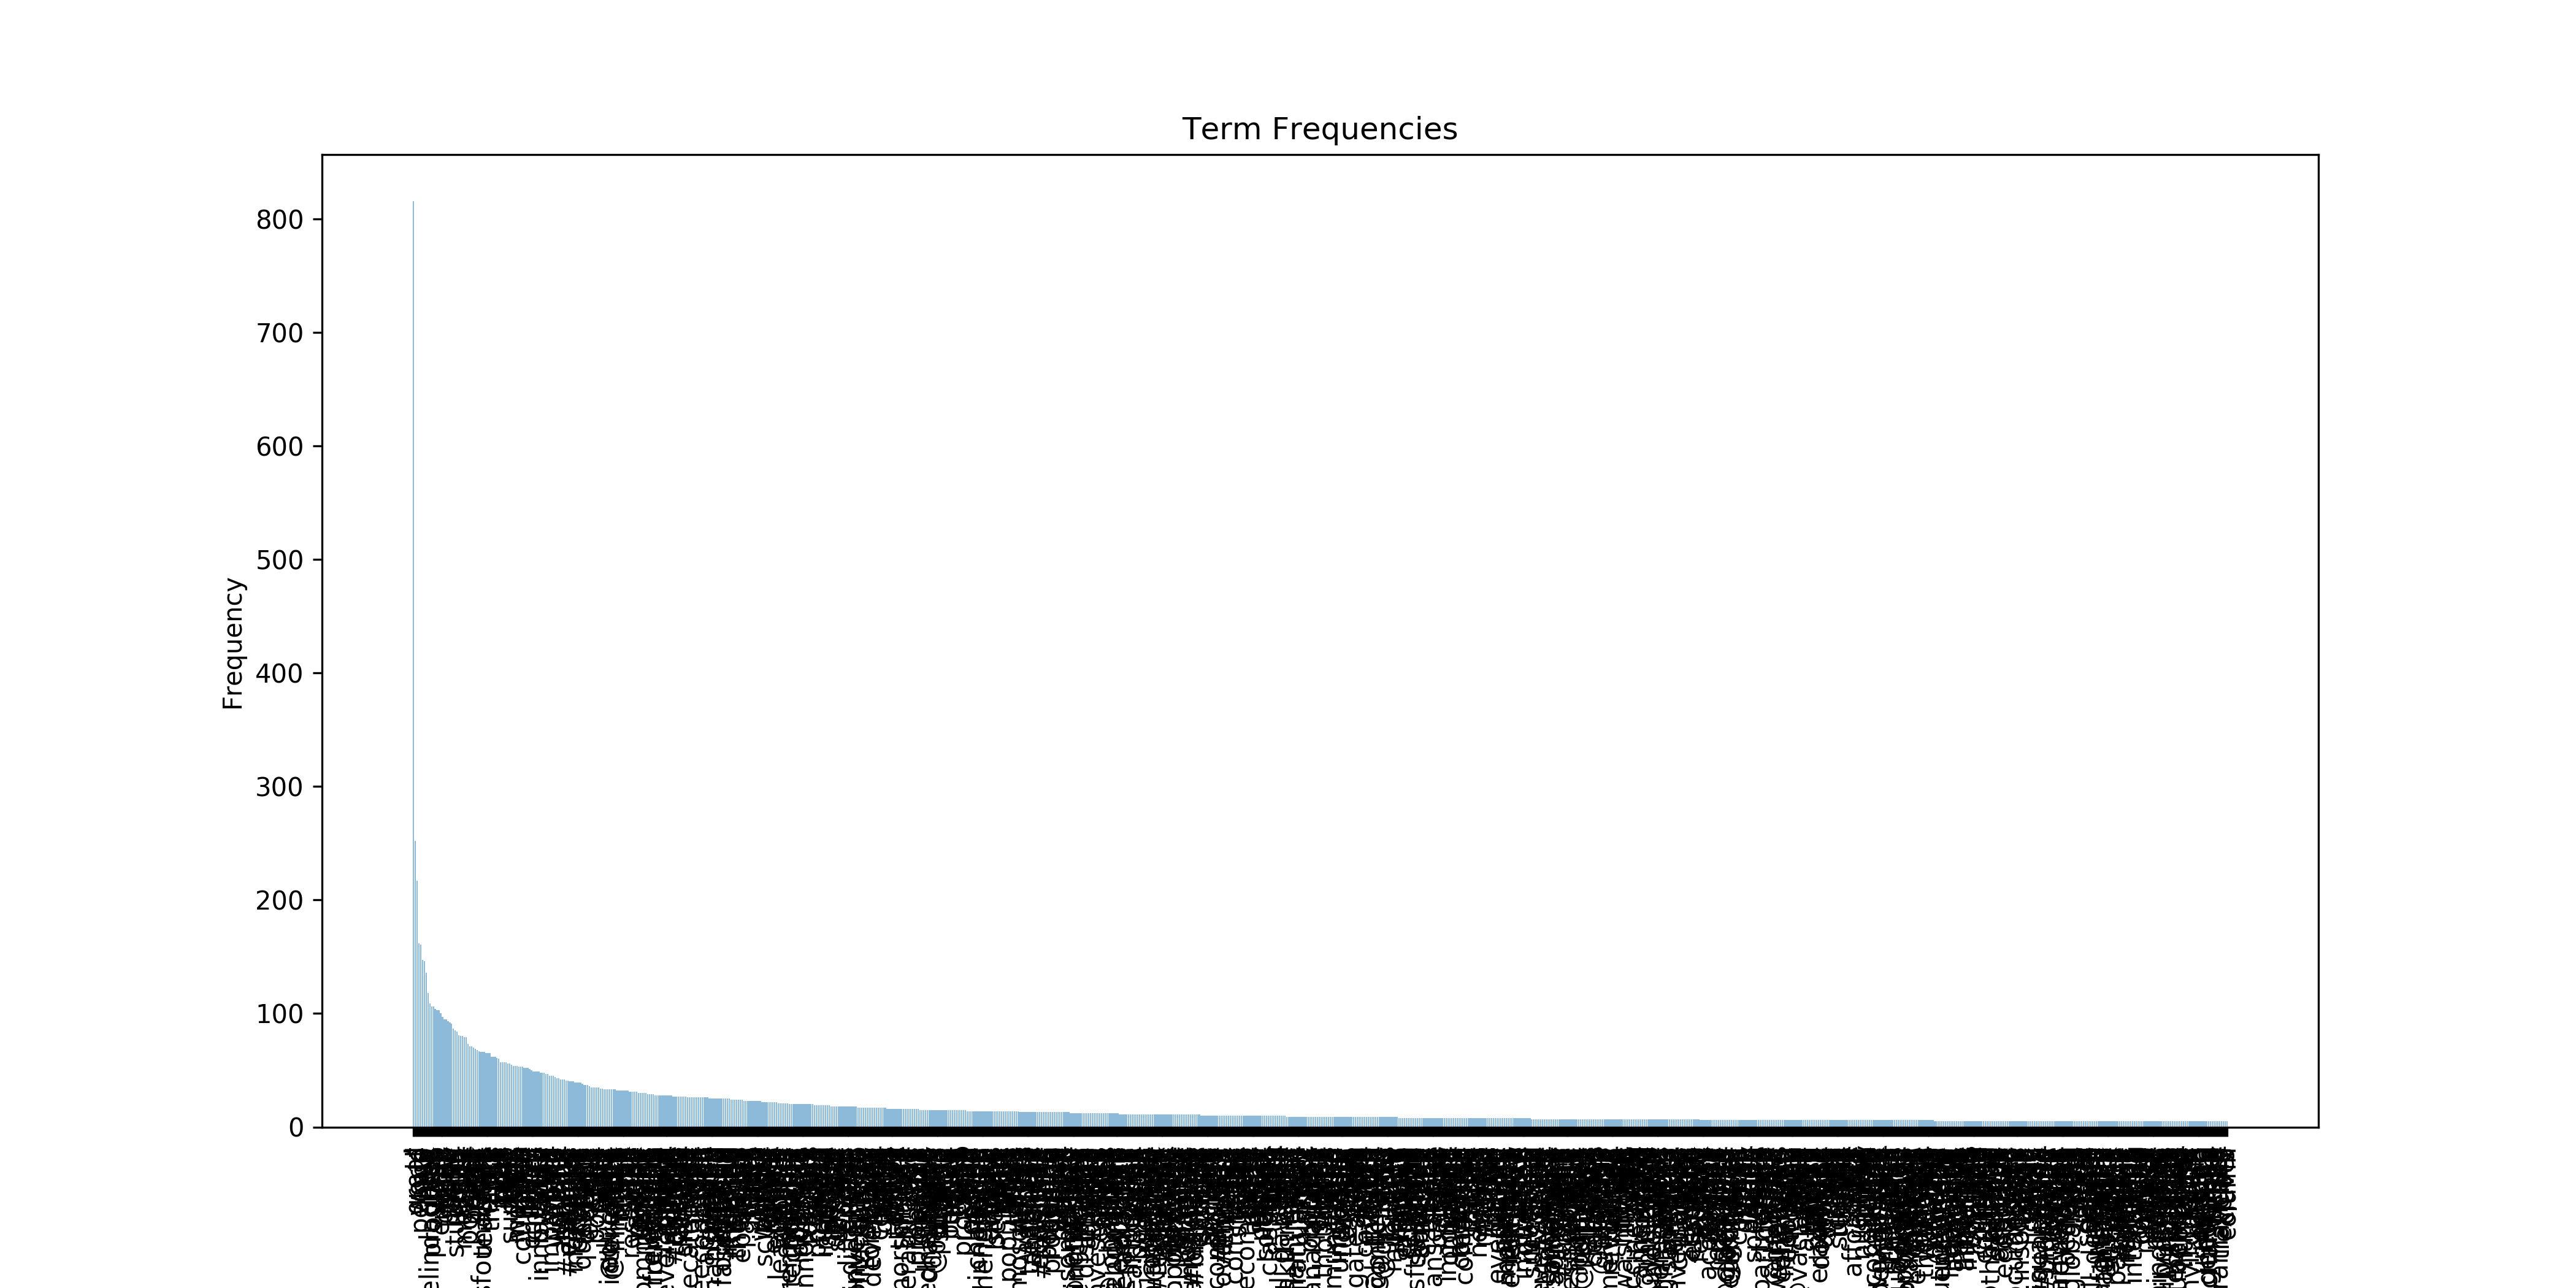
\includegraphics[width=\textwidth]{res/img/term_distribution}
\caption{Term distribution}
\end{figure}

\begin{figure}[!htpb]
\centering
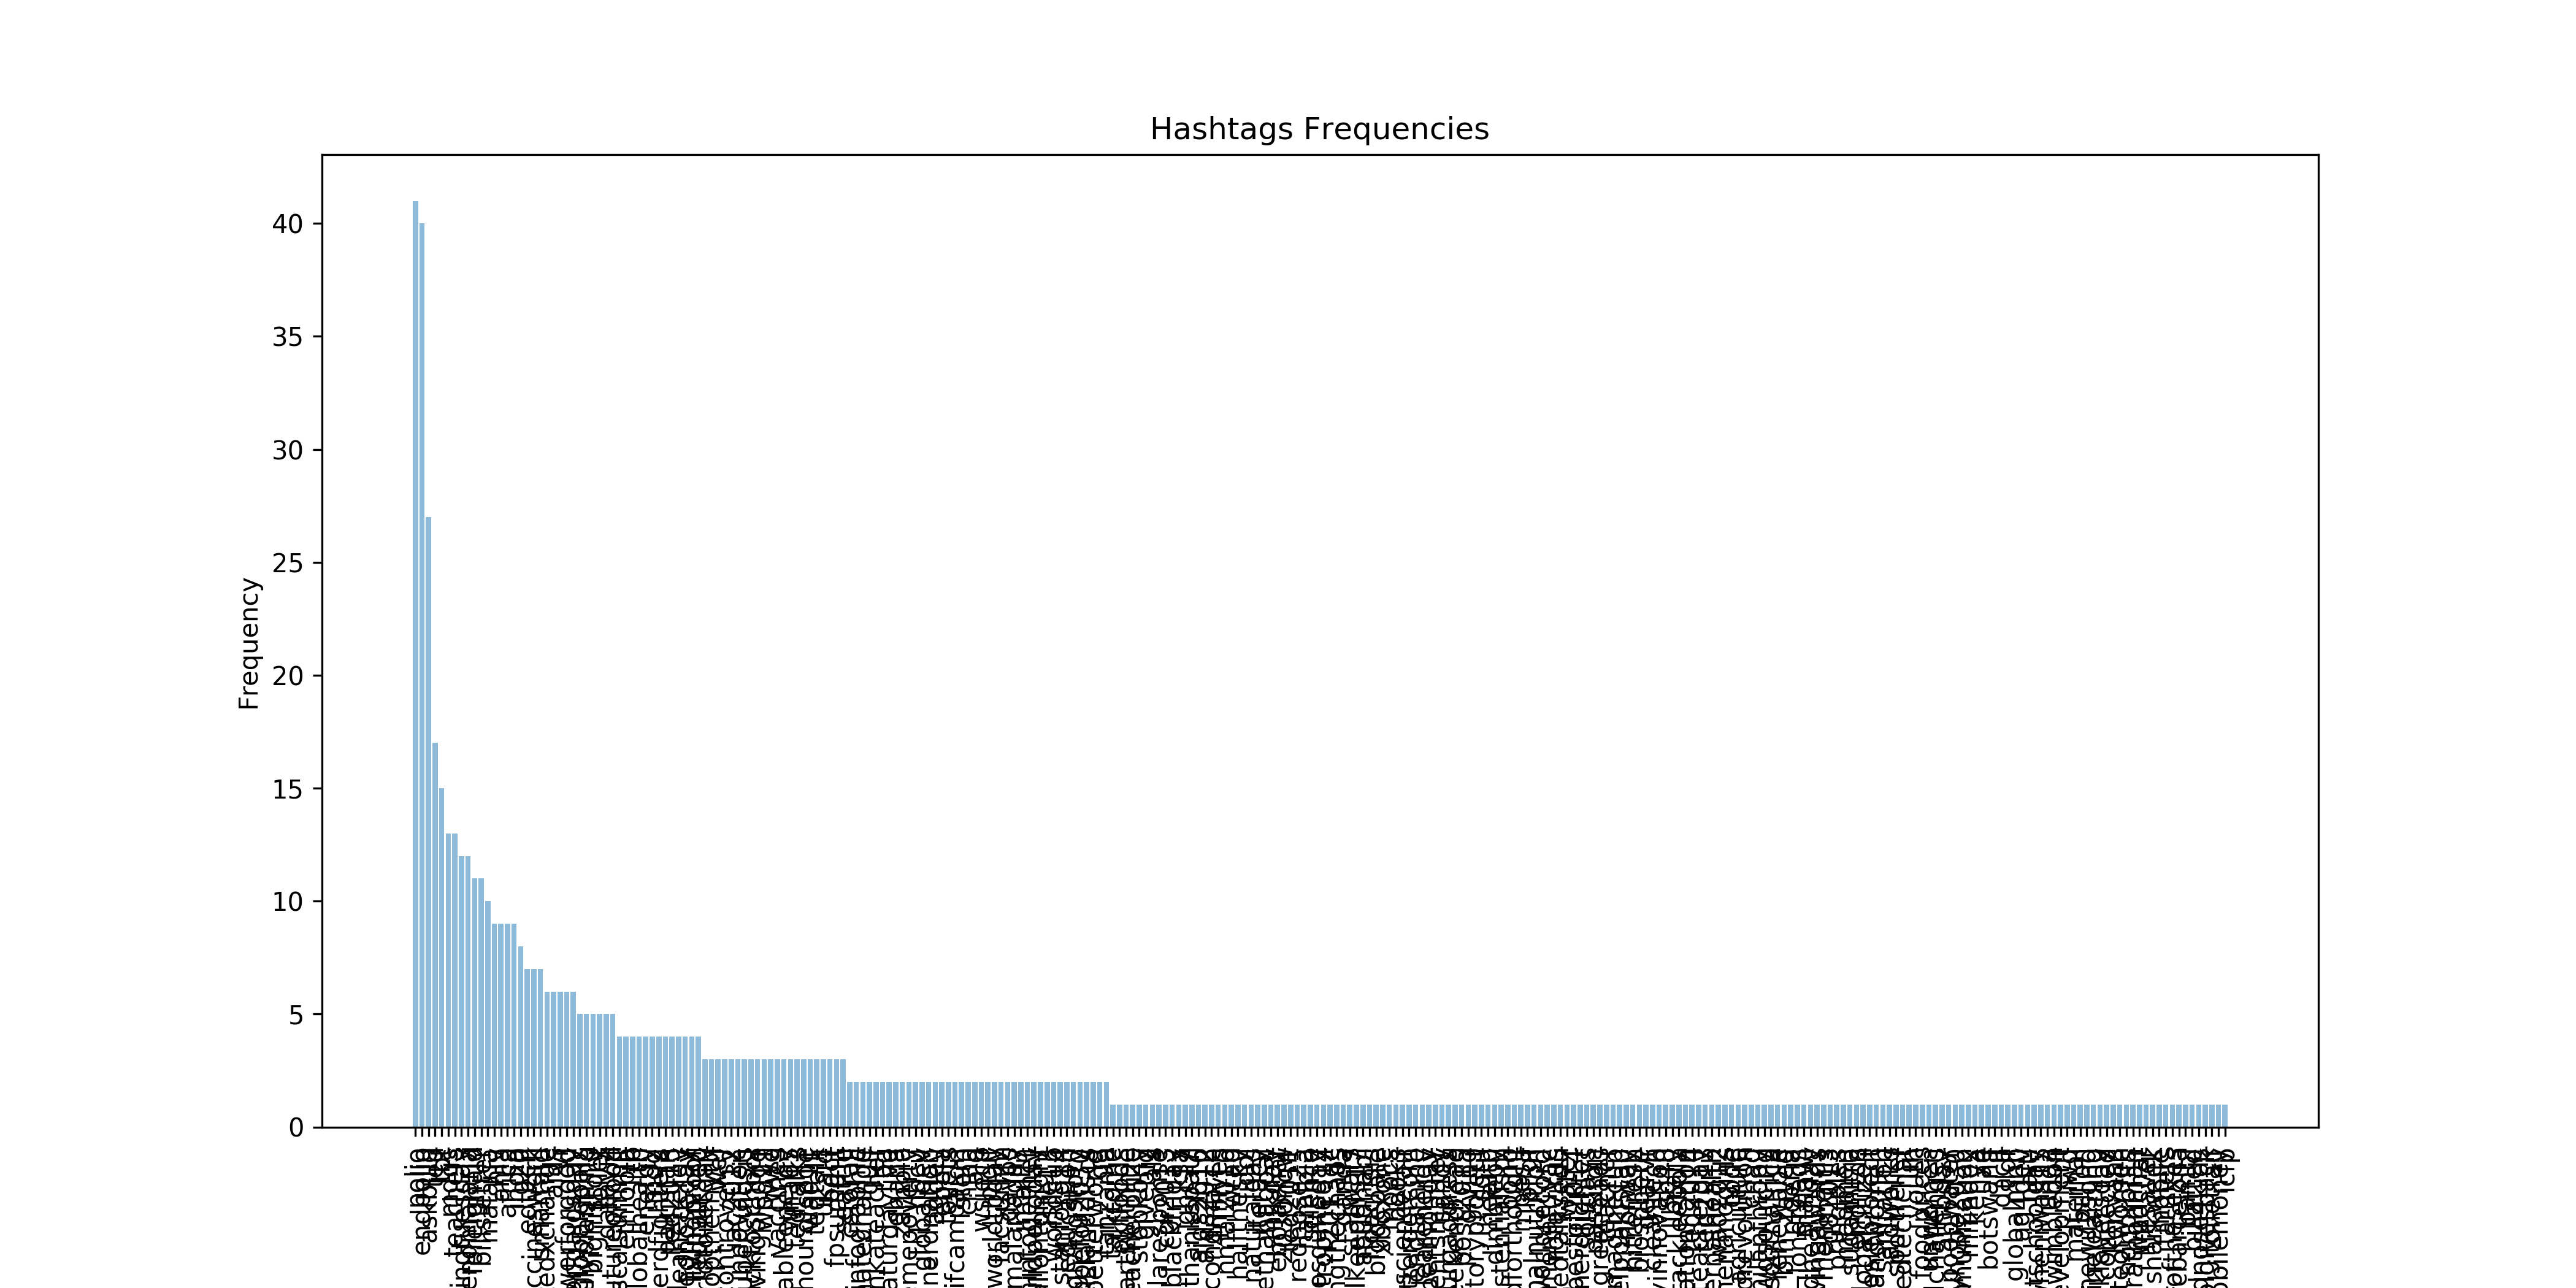
\includegraphics[width=\textwidth]{res/img/hashtags_distribution}
\caption{Hashtag distribution}
\end{figure}

\subsection{Activity 3}

My query is \emph{polio OR malaria}. Looking at the function \emph{CustomListener} and \emph{format\_filename} I can say that the results are going to be saved in a file named \emph{stream\_polio\_malaria.jsonl}.

\subsection{Activity 4}

Positive tweets:

\begin{enumerate}
\item RT @Lin_Manuel: Gmorning! Happy #GivingTuesday. If you don't have a dollar to give, you STILL have your time, your focus, your voice. Be g...

\item I'm amazed by how @NandanNilekani has lent his entrepreneurial passion to philanthropy. I'm delighted to welcome hi... \url{https://t.co/ly8PPvKz98}

\item I really enjoyed this conversation between our foundation CEO @SueDHellmann and Science Friday host @iraflatow. \url{https://t.co/xRfOtBumhg}

\item @johngreen Congrats @johngreen. I'm excited for you and your readers - including my daughter Phoebe, who's one of your biggest fans!

\item I always learn a lot from my friend @RayDalio. His new book #Principles is a remarkable look at his life and career: \url{https://t.co/2A4EREQLYU}
\end{enumerate}

Negative tweets:

\begin{enumerate}
\item "The death that didn't happen is not visible. A fascinating conversation between @Atul_Gawande and @Gladwell. https://t.co/lLprByfc0u

\item I'm very disappointed with today's decision to end #DACA. Our statement: https://t.co/67YQGYtDGo

\item Melinda and I are deeply saddened to learn that our friend, mentor, and advisor Sam Dryden died this morning. https://t.co/KnAhrA3Czh

\item There has been incredible progress since the last Ebola outbreak. This is why we can't let up... https://t.co/BWE2PG6ZFi

\item 5/ I also have one big regret: When I left school, I knew little about the world's worst inequities. Took me decades to learn.
\end{enumerate}

\end{document}
